% Created by tikzDevice version 0.12.3.1 on 2022-04-28 16:23:18
% !TEX encoding = UTF-8 Unicode
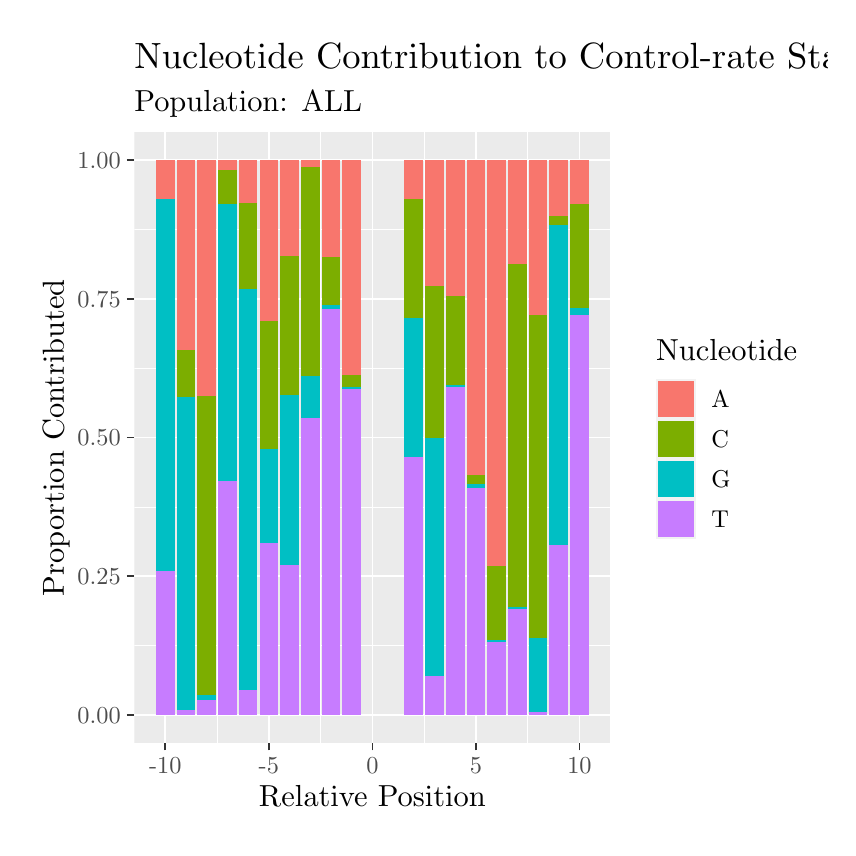
\begin{tikzpicture}[x=1pt,y=1pt]
\definecolor{fillColor}{RGB}{255,255,255}
\path[use as bounding box,fill=fillColor,fill opacity=0.00] (0,0) rectangle (289.08,289.08);
\begin{scope}
\path[clip] (  0.00,  0.00) rectangle (289.08,289.08);
\definecolor{drawColor}{RGB}{255,255,255}
\definecolor{fillColor}{RGB}{255,255,255}

\path[draw=drawColor,line width= 0.6pt,line join=round,line cap=round,fill=fillColor] (  0.00,  0.00) rectangle (289.08,289.08);
\end{scope}
\begin{scope}
\path[clip] ( 38.56, 30.69) rectangle (210.56,251.21);
\definecolor{fillColor}{gray}{0.92}

\path[fill=fillColor] ( 38.56, 30.69) rectangle (210.56,251.21);
\definecolor{drawColor}{RGB}{255,255,255}

\path[draw=drawColor,line width= 0.3pt,line join=round] ( 38.56, 65.77) --
	(210.56, 65.77);

\path[draw=drawColor,line width= 0.3pt,line join=round] ( 38.56,115.89) --
	(210.56,115.89);

\path[draw=drawColor,line width= 0.3pt,line join=round] ( 38.56,166.01) --
	(210.56,166.01);

\path[draw=drawColor,line width= 0.3pt,line join=round] ( 38.56,216.13) --
	(210.56,216.13);

\path[draw=drawColor,line width= 0.3pt,line join=round] ( 68.45, 30.69) --
	( 68.45,251.21);

\path[draw=drawColor,line width= 0.3pt,line join=round] (105.85, 30.69) --
	(105.85,251.21);

\path[draw=drawColor,line width= 0.3pt,line join=round] (143.26, 30.69) --
	(143.26,251.21);

\path[draw=drawColor,line width= 0.3pt,line join=round] (180.67, 30.69) --
	(180.67,251.21);

\path[draw=drawColor,line width= 0.6pt,line join=round] ( 38.56, 40.71) --
	(210.56, 40.71);

\path[draw=drawColor,line width= 0.6pt,line join=round] ( 38.56, 90.83) --
	(210.56, 90.83);

\path[draw=drawColor,line width= 0.6pt,line join=round] ( 38.56,140.95) --
	(210.56,140.95);

\path[draw=drawColor,line width= 0.6pt,line join=round] ( 38.56,191.07) --
	(210.56,191.07);

\path[draw=drawColor,line width= 0.6pt,line join=round] ( 38.56,241.18) --
	(210.56,241.18);

\path[draw=drawColor,line width= 0.6pt,line join=round] ( 49.74, 30.69) --
	( 49.74,251.21);

\path[draw=drawColor,line width= 0.6pt,line join=round] ( 87.15, 30.69) --
	( 87.15,251.21);

\path[draw=drawColor,line width= 0.6pt,line join=round] (124.56, 30.69) --
	(124.56,251.21);

\path[draw=drawColor,line width= 0.6pt,line join=round] (161.97, 30.69) --
	(161.97,251.21);

\path[draw=drawColor,line width= 0.6pt,line join=round] (199.38, 30.69) --
	(199.38,251.21);
\definecolor{fillColor}{RGB}{248,118,109}

\path[fill=fillColor] ( 46.37,227.21) rectangle ( 53.11,241.18);
\definecolor{fillColor}{RGB}{124,174,0}

\path[fill=fillColor] ( 46.37,227.12) rectangle ( 53.11,227.21);
\definecolor{fillColor}{RGB}{199,124,255}

\path[fill=fillColor] ( 46.37, 40.71) rectangle ( 53.11, 92.91);
\definecolor{fillColor}{RGB}{0,191,196}

\path[fill=fillColor] ( 46.37, 92.91) rectangle ( 53.11,227.12);
\definecolor{fillColor}{RGB}{248,118,109}

\path[fill=fillColor] ( 53.86,172.72) rectangle ( 60.59,241.18);
\definecolor{fillColor}{RGB}{124,174,0}

\path[fill=fillColor] ( 53.86,155.54) rectangle ( 60.59,172.72);
\definecolor{fillColor}{RGB}{199,124,255}

\path[fill=fillColor] ( 53.86, 40.71) rectangle ( 60.59, 42.36);
\definecolor{fillColor}{RGB}{0,191,196}

\path[fill=fillColor] ( 53.86, 42.36) rectangle ( 60.59,155.54);
\definecolor{fillColor}{RGB}{248,118,109}

\path[fill=fillColor] ( 61.34,155.90) rectangle ( 68.07,241.18);
\definecolor{fillColor}{RGB}{124,174,0}

\path[fill=fillColor] ( 61.34, 48.09) rectangle ( 68.07,155.90);
\definecolor{fillColor}{RGB}{199,124,255}

\path[fill=fillColor] ( 61.34, 40.71) rectangle ( 68.07, 46.21);
\definecolor{fillColor}{RGB}{0,191,196}

\path[fill=fillColor] ( 61.34, 46.21) rectangle ( 68.07, 48.09);
\definecolor{fillColor}{RGB}{248,118,109}

\path[fill=fillColor] ( 68.82,237.62) rectangle ( 75.55,241.18);
\definecolor{fillColor}{RGB}{124,174,0}

\path[fill=fillColor] ( 68.82,225.20) rectangle ( 75.55,237.62);
\definecolor{fillColor}{RGB}{199,124,255}

\path[fill=fillColor] ( 68.82, 40.71) rectangle ( 75.55,125.22);
\definecolor{fillColor}{RGB}{0,191,196}

\path[fill=fillColor] ( 68.82,125.22) rectangle ( 75.55,225.20);
\definecolor{fillColor}{RGB}{248,118,109}

\path[fill=fillColor] ( 76.30,225.88) rectangle ( 83.04,241.18);
\definecolor{fillColor}{RGB}{124,174,0}

\path[fill=fillColor] ( 76.30,194.71) rectangle ( 83.04,225.88);
\definecolor{fillColor}{RGB}{0,191,196}

\path[fill=fillColor] ( 76.30, 49.66) rectangle ( 83.04,194.71);
\definecolor{fillColor}{RGB}{199,124,255}

\path[fill=fillColor] ( 76.30, 40.71) rectangle ( 83.04, 49.66);
\definecolor{fillColor}{RGB}{248,118,109}

\path[fill=fillColor] ( 83.78,183.05) rectangle ( 90.52,241.18);
\definecolor{fillColor}{RGB}{124,174,0}

\path[fill=fillColor] ( 83.78,136.77) rectangle ( 90.52,183.05);
\definecolor{fillColor}{RGB}{0,191,196}

\path[fill=fillColor] ( 83.78,103.04) rectangle ( 90.52,136.77);
\definecolor{fillColor}{RGB}{199,124,255}

\path[fill=fillColor] ( 83.78, 40.71) rectangle ( 90.52,103.04);
\definecolor{fillColor}{RGB}{248,118,109}

\path[fill=fillColor] ( 91.27,206.59) rectangle ( 98.00,241.18);
\definecolor{fillColor}{RGB}{124,174,0}

\path[fill=fillColor] ( 91.27,156.46) rectangle ( 98.00,206.59);
\definecolor{fillColor}{RGB}{199,124,255}

\path[fill=fillColor] ( 91.27, 40.71) rectangle ( 98.00, 95.03);
\definecolor{fillColor}{RGB}{0,191,196}

\path[fill=fillColor] ( 91.27, 95.03) rectangle ( 98.00,156.46);
\definecolor{fillColor}{RGB}{248,118,109}

\path[fill=fillColor] ( 98.75,238.79) rectangle (105.48,241.18);
\definecolor{fillColor}{RGB}{124,174,0}

\path[fill=fillColor] ( 98.75,163.21) rectangle (105.48,238.79);
\definecolor{fillColor}{RGB}{0,191,196}

\path[fill=fillColor] ( 98.75,148.06) rectangle (105.48,163.21);
\definecolor{fillColor}{RGB}{199,124,255}

\path[fill=fillColor] ( 98.75, 40.71) rectangle (105.48,148.06);
\definecolor{fillColor}{RGB}{248,118,109}

\path[fill=fillColor] (106.23,206.27) rectangle (112.96,241.18);
\definecolor{fillColor}{RGB}{124,174,0}

\path[fill=fillColor] (106.23,188.72) rectangle (112.96,206.27);
\definecolor{fillColor}{RGB}{199,124,255}

\path[fill=fillColor] (106.23, 40.71) rectangle (112.96,187.25);
\definecolor{fillColor}{RGB}{0,191,196}

\path[fill=fillColor] (106.23,187.25) rectangle (112.96,188.72);
\definecolor{fillColor}{RGB}{248,118,109}

\path[fill=fillColor] (113.71,163.52) rectangle (120.44,241.18);
\definecolor{fillColor}{RGB}{124,174,0}

\path[fill=fillColor] (113.71,159.18) rectangle (120.44,163.52);
\definecolor{fillColor}{RGB}{0,191,196}

\path[fill=fillColor] (113.71,158.42) rectangle (120.44,159.18);
\definecolor{fillColor}{RGB}{199,124,255}

\path[fill=fillColor] (113.71, 40.71) rectangle (120.44,158.42);
\definecolor{fillColor}{RGB}{248,118,109}

\path[fill=fillColor] (136.16,227.26) rectangle (142.89,241.18);
\definecolor{fillColor}{RGB}{124,174,0}

\path[fill=fillColor] (136.16,184.13) rectangle (142.89,227.26);
\definecolor{fillColor}{RGB}{199,124,255}

\path[fill=fillColor] (136.16, 40.71) rectangle (142.89,133.79);
\definecolor{fillColor}{RGB}{0,191,196}

\path[fill=fillColor] (136.16,133.79) rectangle (142.89,184.13);
\definecolor{fillColor}{RGB}{248,118,109}

\path[fill=fillColor] (143.64,195.62) rectangle (150.37,241.18);
\definecolor{fillColor}{RGB}{124,174,0}

\path[fill=fillColor] (143.64,140.96) rectangle (150.37,195.62);
\definecolor{fillColor}{RGB}{0,191,196}

\path[fill=fillColor] (143.64, 54.69) rectangle (150.37,140.96);
\definecolor{fillColor}{RGB}{199,124,255}

\path[fill=fillColor] (143.64, 40.71) rectangle (150.37, 54.69);
\definecolor{fillColor}{RGB}{248,118,109}

\path[fill=fillColor] (151.12,192.18) rectangle (157.85,241.18);
\definecolor{fillColor}{RGB}{124,174,0}

\path[fill=fillColor] (151.12,160.06) rectangle (157.85,192.18);
\definecolor{fillColor}{RGB}{199,124,255}

\path[fill=fillColor] (151.12, 40.71) rectangle (157.85,159.22);
\definecolor{fillColor}{RGB}{0,191,196}

\path[fill=fillColor] (151.12,159.22) rectangle (157.85,160.06);
\definecolor{fillColor}{RGB}{248,118,109}

\path[fill=fillColor] (158.60,127.35) rectangle (165.34,241.18);
\definecolor{fillColor}{RGB}{124,174,0}

\path[fill=fillColor] (158.60,124.09) rectangle (165.34,127.35);
\definecolor{fillColor}{RGB}{199,124,255}

\path[fill=fillColor] (158.60, 40.71) rectangle (165.34,122.65);
\definecolor{fillColor}{RGB}{0,191,196}

\path[fill=fillColor] (158.60,122.65) rectangle (165.34,124.09);
\definecolor{fillColor}{RGB}{248,118,109}

\path[fill=fillColor] (166.08, 94.69) rectangle (172.82,241.18);
\definecolor{fillColor}{RGB}{124,174,0}

\path[fill=fillColor] (166.08, 67.82) rectangle (172.82, 94.69);
\definecolor{fillColor}{RGB}{0,191,196}

\path[fill=fillColor] (166.08, 67.05) rectangle (172.82, 67.82);
\definecolor{fillColor}{RGB}{199,124,255}

\path[fill=fillColor] (166.08, 40.71) rectangle (172.82, 67.05);
\definecolor{fillColor}{RGB}{248,118,109}

\path[fill=fillColor] (173.57,203.68) rectangle (180.30,241.18);
\definecolor{fillColor}{RGB}{124,174,0}

\path[fill=fillColor] (173.57, 79.89) rectangle (180.30,203.68);
\definecolor{fillColor}{RGB}{0,191,196}

\path[fill=fillColor] (173.57, 78.89) rectangle (180.30, 79.89);
\definecolor{fillColor}{RGB}{199,124,255}

\path[fill=fillColor] (173.57, 40.71) rectangle (180.30, 78.89);
\definecolor{fillColor}{RGB}{248,118,109}

\path[fill=fillColor] (181.05,185.43) rectangle (187.78,241.18);
\definecolor{fillColor}{RGB}{124,174,0}

\path[fill=fillColor] (181.05, 68.54) rectangle (187.78,185.43);
\definecolor{fillColor}{RGB}{199,124,255}

\path[fill=fillColor] (181.05, 40.71) rectangle (187.78, 41.68);
\definecolor{fillColor}{RGB}{0,191,196}

\path[fill=fillColor] (181.05, 41.68) rectangle (187.78, 68.54);
\definecolor{fillColor}{RGB}{248,118,109}

\path[fill=fillColor] (188.53,220.89) rectangle (195.26,241.18);
\definecolor{fillColor}{RGB}{124,174,0}

\path[fill=fillColor] (188.53,217.89) rectangle (195.26,220.89);
\definecolor{fillColor}{RGB}{199,124,255}

\path[fill=fillColor] (188.53, 40.71) rectangle (195.26,102.00);
\definecolor{fillColor}{RGB}{0,191,196}

\path[fill=fillColor] (188.53,102.00) rectangle (195.26,217.89);
\definecolor{fillColor}{RGB}{248,118,109}

\path[fill=fillColor] (196.01,225.20) rectangle (202.75,241.18);
\definecolor{fillColor}{RGB}{124,174,0}

\path[fill=fillColor] (196.01,187.92) rectangle (202.75,225.20);
\definecolor{fillColor}{RGB}{0,191,196}

\path[fill=fillColor] (196.01,185.18) rectangle (202.75,187.92);
\definecolor{fillColor}{RGB}{199,124,255}

\path[fill=fillColor] (196.01, 40.71) rectangle (202.75,185.18);
\end{scope}
\begin{scope}
\path[clip] (  0.00,  0.00) rectangle (289.08,289.08);
\definecolor{drawColor}{gray}{0.30}

\node[text=drawColor,anchor=base east,inner sep=0pt, outer sep=0pt, scale=  0.88] at ( 33.61, 37.68) {0.00};

\node[text=drawColor,anchor=base east,inner sep=0pt, outer sep=0pt, scale=  0.88] at ( 33.61, 87.80) {0.25};

\node[text=drawColor,anchor=base east,inner sep=0pt, outer sep=0pt, scale=  0.88] at ( 33.61,137.92) {0.50};

\node[text=drawColor,anchor=base east,inner sep=0pt, outer sep=0pt, scale=  0.88] at ( 33.61,188.04) {0.75};

\node[text=drawColor,anchor=base east,inner sep=0pt, outer sep=0pt, scale=  0.88] at ( 33.61,238.15) {1.00};
\end{scope}
\begin{scope}
\path[clip] (  0.00,  0.00) rectangle (289.08,289.08);
\definecolor{drawColor}{gray}{0.20}

\path[draw=drawColor,line width= 0.6pt,line join=round] ( 35.81, 40.71) --
	( 38.56, 40.71);

\path[draw=drawColor,line width= 0.6pt,line join=round] ( 35.81, 90.83) --
	( 38.56, 90.83);

\path[draw=drawColor,line width= 0.6pt,line join=round] ( 35.81,140.95) --
	( 38.56,140.95);

\path[draw=drawColor,line width= 0.6pt,line join=round] ( 35.81,191.07) --
	( 38.56,191.07);

\path[draw=drawColor,line width= 0.6pt,line join=round] ( 35.81,241.18) --
	( 38.56,241.18);
\end{scope}
\begin{scope}
\path[clip] (  0.00,  0.00) rectangle (289.08,289.08);
\definecolor{drawColor}{gray}{0.20}

\path[draw=drawColor,line width= 0.6pt,line join=round] ( 49.74, 27.94) --
	( 49.74, 30.69);

\path[draw=drawColor,line width= 0.6pt,line join=round] ( 87.15, 27.94) --
	( 87.15, 30.69);

\path[draw=drawColor,line width= 0.6pt,line join=round] (124.56, 27.94) --
	(124.56, 30.69);

\path[draw=drawColor,line width= 0.6pt,line join=round] (161.97, 27.94) --
	(161.97, 30.69);

\path[draw=drawColor,line width= 0.6pt,line join=round] (199.38, 27.94) --
	(199.38, 30.69);
\end{scope}
\begin{scope}
\path[clip] (  0.00,  0.00) rectangle (289.08,289.08);
\definecolor{drawColor}{gray}{0.30}

\node[text=drawColor,anchor=base,inner sep=0pt, outer sep=0pt, scale=  0.88] at ( 49.74, 19.68) {-10};

\node[text=drawColor,anchor=base,inner sep=0pt, outer sep=0pt, scale=  0.88] at ( 87.15, 19.68) {-5};

\node[text=drawColor,anchor=base,inner sep=0pt, outer sep=0pt, scale=  0.88] at (124.56, 19.68) {0};

\node[text=drawColor,anchor=base,inner sep=0pt, outer sep=0pt, scale=  0.88] at (161.97, 19.68) {5};

\node[text=drawColor,anchor=base,inner sep=0pt, outer sep=0pt, scale=  0.88] at (199.38, 19.68) {10};
\end{scope}
\begin{scope}
\path[clip] (  0.00,  0.00) rectangle (289.08,289.08);
\definecolor{drawColor}{RGB}{0,0,0}

\node[text=drawColor,anchor=base,inner sep=0pt, outer sep=0pt, scale=  1.10] at (124.56,  7.64) {Relative Position};
\end{scope}
\begin{scope}
\path[clip] (  0.00,  0.00) rectangle (289.08,289.08);
\definecolor{drawColor}{RGB}{0,0,0}

\node[text=drawColor,rotate= 90.00,anchor=base,inner sep=0pt, outer sep=0pt, scale=  1.10] at ( 13.08,140.95) {Proportion Contributed};
\end{scope}
\begin{scope}
\path[clip] (  0.00,  0.00) rectangle (289.08,289.08);
\definecolor{fillColor}{RGB}{255,255,255}

\path[fill=fillColor] (221.56, 98.93) rectangle (283.58,182.96);
\end{scope}
\begin{scope}
\path[clip] (  0.00,  0.00) rectangle (289.08,289.08);
\definecolor{drawColor}{RGB}{0,0,0}

\node[text=drawColor,anchor=base west,inner sep=0pt, outer sep=0pt, scale=  1.10] at (227.06,168.82) {Nucleotide};
\end{scope}
\begin{scope}
\path[clip] (  0.00,  0.00) rectangle (289.08,289.08);
\definecolor{fillColor}{gray}{0.95}

\path[fill=fillColor] (227.06,147.79) rectangle (241.52,162.25);
\end{scope}
\begin{scope}
\path[clip] (  0.00,  0.00) rectangle (289.08,289.08);
\definecolor{fillColor}{RGB}{248,118,109}

\path[fill=fillColor] (227.78,148.51) rectangle (240.81,161.54);
\end{scope}
\begin{scope}
\path[clip] (  0.00,  0.00) rectangle (289.08,289.08);
\definecolor{fillColor}{gray}{0.95}

\path[fill=fillColor] (227.06,133.34) rectangle (241.52,147.79);
\end{scope}
\begin{scope}
\path[clip] (  0.00,  0.00) rectangle (289.08,289.08);
\definecolor{fillColor}{RGB}{124,174,0}

\path[fill=fillColor] (227.78,134.05) rectangle (240.81,147.08);
\end{scope}
\begin{scope}
\path[clip] (  0.00,  0.00) rectangle (289.08,289.08);
\definecolor{fillColor}{gray}{0.95}

\path[fill=fillColor] (227.06,118.89) rectangle (241.52,133.34);
\end{scope}
\begin{scope}
\path[clip] (  0.00,  0.00) rectangle (289.08,289.08);
\definecolor{fillColor}{RGB}{0,191,196}

\path[fill=fillColor] (227.78,119.60) rectangle (240.81,132.63);
\end{scope}
\begin{scope}
\path[clip] (  0.00,  0.00) rectangle (289.08,289.08);
\definecolor{fillColor}{gray}{0.95}

\path[fill=fillColor] (227.06,104.43) rectangle (241.52,118.89);
\end{scope}
\begin{scope}
\path[clip] (  0.00,  0.00) rectangle (289.08,289.08);
\definecolor{fillColor}{RGB}{199,124,255}

\path[fill=fillColor] (227.78,105.14) rectangle (240.81,118.17);
\end{scope}
\begin{scope}
\path[clip] (  0.00,  0.00) rectangle (289.08,289.08);
\definecolor{drawColor}{RGB}{0,0,0}

\node[text=drawColor,anchor=base west,inner sep=0pt, outer sep=0pt, scale=  0.88] at (247.02,151.99) {A};
\end{scope}
\begin{scope}
\path[clip] (  0.00,  0.00) rectangle (289.08,289.08);
\definecolor{drawColor}{RGB}{0,0,0}

\node[text=drawColor,anchor=base west,inner sep=0pt, outer sep=0pt, scale=  0.88] at (247.02,137.54) {C};
\end{scope}
\begin{scope}
\path[clip] (  0.00,  0.00) rectangle (289.08,289.08);
\definecolor{drawColor}{RGB}{0,0,0}

\node[text=drawColor,anchor=base west,inner sep=0pt, outer sep=0pt, scale=  0.88] at (247.02,123.08) {G};
\end{scope}
\begin{scope}
\path[clip] (  0.00,  0.00) rectangle (289.08,289.08);
\definecolor{drawColor}{RGB}{0,0,0}

\node[text=drawColor,anchor=base west,inner sep=0pt, outer sep=0pt, scale=  0.88] at (247.02,108.63) {T};
\end{scope}
\begin{scope}
\path[clip] (  0.00,  0.00) rectangle (289.08,289.08);
\definecolor{drawColor}{RGB}{0,0,0}

\node[text=drawColor,anchor=base west,inner sep=0pt, outer sep=0pt, scale=  1.10] at ( 38.56,258.85) {Population: ALL};
\end{scope}
\begin{scope}
\path[clip] (  0.00,  0.00) rectangle (289.08,289.08);
\definecolor{drawColor}{RGB}{0,0,0}

\node[text=drawColor,anchor=base west,inner sep=0pt, outer sep=0pt, scale=  1.32] at ( 38.56,274.49) {Nucleotide Contribution to Control-rate Statistic: cpg-GC-AT};
\end{scope}
\end{tikzpicture}
